\documentclass{beamer}
\usepackage{graphicx}
\usepackage[utf8]{inputenc}
\usepackage{biblatex}
\setbeamercovered{transparent=15}
\addbibresource{../bibliography.bib}

\setbeamerfont{institute}{size=\large}
\setbeamerfont{date}{size=\small}

\newcommand\red[1]{\textcolor{red}{#1}}

\usetheme{Madrid}
\usecolortheme{orchid}

\title{Blockchain and Bitcoin}
\subtitle[]{Overview of Blockchain technology and cryptocurrencies, focusing on
the Bitcoin protocol and its scalability and privacy aspects}
\institute[]{Università degli studi di Brescia}
\author{Michele Zanotti}
\date{\today}

\begin{document}
  \begin{frame}
    \titlepage
  \end{frame}
  \begin{frame}{Summary}
    \tableofcontents
  \end{frame}

  %%%%%%%%%%%%%%%%%%%%%
  %%% FIRST SECTION %%%
  %%%%%%%%%%%%%%%%%%%%%
  \section{Introduction}
  \begin{frame}{Introduction}
    \framesubtitle{Distributed systems}
    \begin{columns}[onlytextwidth]
      \column{.5\textwidth} \begin{block}{Distributed system}
        A \textcolor{red}{distributed system} is a network that consists of autonomous nodes,
        connected using a distribution middleware, which acts in a coordinated way
        (passing messages to each other) in order to achieve a common outcome and
        that can be seen by the user as a single logical platform.
      \end{block}

      \column{.5\textwidth}\begin{figure}[!htb]
        \centering
        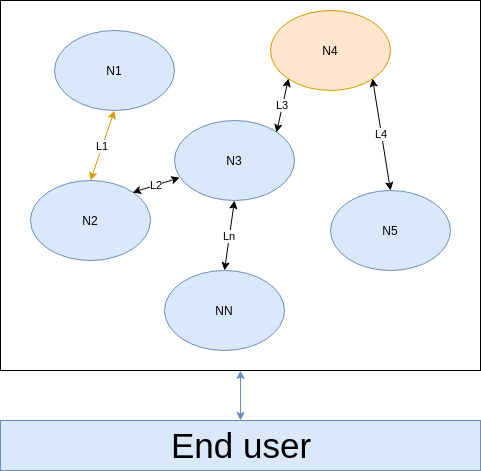
\includegraphics[width=0.7\linewidth]{../img/distributed-system.png}
      \end{figure}
    \end{columns}
  \end{frame}




  \begin{frame}{Introduction}
    \framesubtitle{Distributed systems}
      The desired properties of a distributed system are the following:\vspace{10pt}
      \begin{itemize}
        \item \textbf{Consistency}: all the nodes have the same lates available copy of the data.
        \item \textbf{Availability}: the system is always working and responding to the
        input requests without any failures.
        \item \textbf{Partition tolerance}: if a group of nodes fails the distributed system
        still continues to operate correctly
      \end{itemize}
  \end{frame}




  \begin{frame}{Introduction}
    \framesubtitle{Distributed systems}
    Even if some of the nodes fault or links break, a distributed system should tolerate
    this and should continue to work correctly. There are two types of fault:
    \begin{itemize}
      \item Simple node crash
      \item Exhibition of malicious or inconsistent behavior arbitrarily: \red{Byzantine fault}
    \end{itemize}

    \begin{block}{Byzantine nodes}
      A \textcolor{red}{Byzantine node} is a node that has an arbitrary behavior,
      which can even be malicious.
    \end{block}
  \end{frame}




  \begin{frame}{Introduction}
    \framesubtitle{Distributed systems}
    \begin{block}{Consensus}
      \red{Consensus} is the process of agreement between untrusted nodes on a data
      value.
    \end{block}

    Consensus mechanism requirements:
    \begin{itemize}
      \item \textbf{Agreement}: non-byzantine nodes must agree on the same value
      \item \textbf{Termination}: the consensus process must come to an end (nodes
      have to reach a decision)
      \item \textbf{Validity}: the agreed value must have been proposed by at
      least one honest node
      \item \textbf{Fault tolerance}: the consensus algorithm must work even
      in the presence of one or more Byzantine nodes
    \end{itemize}
  \end{frame}



  \begin{frame}{Introduction}
    \framesubtitle{Distributed systems}
    \begin{block}{The Byzantine generals problem}
      \begin{itemize}
        \item Problem formulated by Leslie Lamport \cite{lamport1982byzantine}
        \item A group of generals are surrounding a city and they have to agree
        on a common decision: attack or retreat.
        \item Their only communication way is a messenger
        \item Some of the generals may be \emph{traitors}: they communicate
        misleading message for preventing the loyal generals from reaching an
        agreement
        \item Requirement: algorithm that allows the loyal generals to agree
        on the same plan regardless of traitors general
      \end{itemize}
    \end{block}
  \end{frame}







  %%%%%%%%%%%%%%%%%%%%%
  %%% SECOND SECTION %%%
  %%%%%%%%%%%%%%%%%%%%%
  \section{Blockchain}
  \begin{frame}{Introduction to Blockchain}
    \framesubtitle{What is Blockchain}

    \begin{block}{Business definition}
      Blockchain is a platform whereby peers can exchange values without the need
      for a central trusted party by using transactions which are stored inside
      the platform in a verifiable and permanent way.
    \end{block}

    \begin{block}{Technical definition}
      Blockchain is a distributed ledger that is
      \begin{itemize}
        \item cryptographically secure
        \item append-only
        \item immutable (extremely hard to change)
        \item updateable only via consensus among nodes
      \end{itemize}
    \end{block}
  \end{frame}




  \begin{frame}[allowframebreaks]{Introduction to Blockchain}
    \framesubtitle{Blockchain features}

    \begin{itemize}
      \item \textbf{Decentralization}: no need of a central trusted entity
      which stores the data and validates the transaction, the same copy of the
      Blockchain is stored by every node and the validation of transaction is
      achieved through consensus \pause
      \item \textbf{Distributed consensus}: Blockchain has high Byzantine Fault
      Tolerance and allows to have a single version of a data value agreed by all
      parties through a consensus algorithm \pause
      \item \textbf{High availability}: Blockchain is based on a peer-to-peer
      network and data replicated on each node: even if one or more nodes fail
      the whole network can continue to work correctly \pause
      \item \textbf{Immutability}: once a block has been added to the blockchain,
      changing it is computationally infeasible \pause
      \item \textbf{Transparency}: every node can see what is in the blockchain \pause
      \item \textbf{Security}: \pause
      \item \textbf{Uniqueness}:
    \end{itemize}
  \end{frame}











  \begin{frame}{References}
    \printbibliography
  \end{frame}

\end{document}
